\mfpicnumber{1}

\opengraphsfile{Parabolas}

\setcounter{footnote}{0}

\label{Parabolas}

We have already learned that the graph of a quadratic function $f(x) = ax^2 + bx + c$ ($a \neq 0$) is called a \textbf{parabola}.  To our surprise and delight, we may also define parabolas in terms of distance.

\medskip

\colorbox{ResultColor}{\bbm

\begin{defn}

\label{paraboladefn}

Let $F$ be a point in the plane and $D$ be a line not containing $F$.   A \index{parabola ! definition of}  \textbf{parabola} is the set of all points equidistant from $F$ and $D$.  The point $F$ is called the \textbf{focus} \index{parabola ! focus} \index{focus (foci) ! of a parabola} of the parabola and the line $D$ is called the \textbf{directrix} \index{parabola ! directrix} \index{directrix ! of a parabola} of the parabola. 

\end{defn}

\ebm}

\medskip

Schematically, we have the following.

\begin{center}

\begin{mfpic}[15]{-7}{7}{0}{5}
\arrow \reverse \arrow \function{-6.25,6.25,0.1}{(x**2)/8}
\dashed \polyline{(0,2), (0,0), (0,-2)}
\dashed \polyline{(0,2), (2, 0.5), (2, -2)}
\dashed \polyline{(0,2), (-2,0.5), (-2, -2)}
\dashed  \polyline{(0,2), (4,2), (4, -2)}
\dashed  \polyline{(0,2), (-4,2), (-4, -2)}
\dashed \polyline{(0,2), (6,4.5), (6, -2)}
\dashed  \polyline{(0,2), (-6,4.5), (-6, -2)}
\plotsymbol[3pt]{Asterisk}{(0, 2)}
\tlabel[cc](0, 2.5){$F$}
\arrow \reverse \arrow \function{-6.5, 6.5, 0.1}{-2}
\tlabel[cc](6.5, -2.5){$D$}
\point[3pt]{(0,0)}
\point[3pt]{(2,0.5)}
\point[3pt]{(-2,0.5)}
\point[3pt]{(4,2)}
\point[3pt]{(-4,2)}
\point[3pt]{(6,4.5)}
\point[3pt]{(-6,4.5)}
\tlabel[cc](0.5,-0.5){$V$}
\end{mfpic}

\end{center}

Each dashed line from the point $F$ to a point on the curve has the same length as the dashed line from the point on the curve to the line $D$.  The point suggestively labeled $V$ is, as you should expect, the \textbf{vertex}.  The \index{parabola ! vertex} \index{vertex ! of a parabola} vertex is the point on the parabola closest to the focus.  

\medskip

We want to use only the distance definition of parabola to derive the equation of a parabola and, if all is right with the universe, we should get an expression much like those studied in Section \ref{QuadraticFunctions}.  Let $p$ denote the directed\footnote{We'll talk more about what `directed' means later.} distance from the vertex to the focus, which by definition is the same as the distance from the vertex to the directrix.  For simplicity, assume that the vertex is $(0,0)$ and that the parabola opens upwards.  Hence, the focus is $(0,p)$ and the directrix is the line $y = -p$.  Our picture becomes 

\begin{center}

\begin{mfpic}[15]{-7}{7}{0}{5}
\axes
\arrow \reverse \arrow \function{-6.25,6.25,0.1}{(x**2)/8}
\plotsymbol[3pt]{Asterisk}{(0, 2)}
\tlabel[cc](0.75, 1.5){$(0,p)$}
\tlabel(7,-0.25){\scriptsize $x$}
\tlabel(0.25,5){\scriptsize $y$}
\arrow \reverse \arrow \function{-6.5, 6.5, 0.1}{-2}
\tlabel[cc](0, -2.5){$y = -p$}
\point[3pt]{(6,4.5)}
\tlabel[cc](7, 3.75){$(x,y)$}
\dashed \polyline{(0,2), (6, 4.5), (6, -2)}
\point[3pt]{(6, -2)}
\point[3pt]{(0,0)}
\tlabel[cc](6, -2.5){$(x, -p)$}
\tlabel[cc](0.5,-0.5){$(0,0)$}
\end{mfpic}

\end{center}

From the definition of parabola, we know the distance from $(0,p)$ to $(x,y)$ is the same as the distance from $(x,-p)$ to $(x,y)$.  Using the Distance Formula, Equation \ref{distanceformula}, we get

\[ \begin{array}{rclr} \sqrt{(x -0)^2 + (y-p)^2} & = & \sqrt{(x-x)^2 + (y - (-p))^2} & \\
\sqrt{x^2 + (y-p)^2} & = & \sqrt{(y+p)^2} & \\
x^2 + (y-p)^2 & = & (y+p)^2 & \mbox{square both sides} \\
x^2 + y^2 - 2py + p^2 & = & y^2 + 2py + p^2 & \mbox{expand quantities} \\
x^2 & = & 4py & \mbox{gather like terms} \\ \end{array} \]

Solving for $y$ yields $y = \frac{x^2}{4p}$, which is a quadratic function of the form found in Equation \ref{vertexofquadraticfunctions} with $a = \frac{1}{4p}$ and vertex $(0, 0)$.

\medskip

We know from previous experience that if the coefficient of $x^2$ is negative, the parabola opens downwards.  In the equation $y = \frac{x^2}{4p}$ this happens when $p < 0$.  In our formulation, we say that $p$ is a `directed distance' from the vertex to the focus:  if $p > 0$, the focus is above the vertex;  if $p < 0$, the focus is below the vertex.   The \index{parabola ! focal length} \index{focal length of a parabola} \textbf{focal length} of a parabola is $|p|$.

\medskip

If we choose to place the vertex at an arbitrary point $(h,k)$, we arrive at the following formula  using either transformations from Section \ref{Transformations} or re-deriving the formula from Definition \ref{paraboladefn}.

\medskip

\colorbox{ResultColor}{\bbm

\begin{eqn}  \label{standardvparabola} \index{parabola ! standard equation ! vertical}  \textbf{The Standard Equation of a Vertical\footnote{That is, a parabola which opens either upwards or downwards.}  Parabola:}  The equation of a (vertical) parabola with vertex $(h,k)$ and focal length $|p|$ is

\[ (x-h)^2 = 4p(y-k) \]

If $p>0$, the parabola opens upwards;  if $p < 0$, it opens downwards.
  
\end{eqn}
  
\ebm}
  
\medskip

Notice that in the standard equation of the parabola above, only one of the variables, $x$, is squared. This is a quick way to distinguish an equation of a parabola from that of a circle because in the equation of a circle, both variables are squared.

\begin{ex} Graph $(x+1)^2 = -8(y-3)$.  Find the vertex, focus, and directrix.

\medskip

{\bf Solution.}  We recognize this as the form given in Equation \ref{standardvparabola}.  Here, $x-h$ is $x+1$ so $h = -1$, and  $y-k$ is $y-3$ so $k = 3$.  Hence, the vertex is $(-1,3)$.  We also see that $4p = -8$ so $p = -2$.  Since $p < 0$, the focus will be below the vertex and the parabola will open downwards. 

\begin{center}

\begin{mfpic}[15]{-7}{5}{-1}{6}
\axes
\xmarks{-6, -5, -4, -3, -2, -1, 0, 1, 2, 3, 4}
\ymarks{0, 1, 2, 3, 4, 5}
\arrow \reverse \arrow \function{-6.5,4.5,0.1}{((x+1)**2)/-8+3}
\plotsymbol[3pt]{Asterisk}{(-1,1)}
\tlabel(5,-0.25){\scriptsize $x$}
\tlabel(0.25,6){\scriptsize $y$}
\point[3pt]{(-1,3)}
\arrow \reverse \arrow \function{-7,5,0.1}{5}
\tlpointsep{4pt}
\scriptsize
\axislabels {x}{{$-6 \hspace{7pt}$} -6, {$-5 \hspace{7pt}$} -5, {$-4 \hspace{7pt}$} -4, {$-3 \hspace{7pt}$} -3, {$-2 \hspace{7pt}$} -2, {$-1 \hspace{7pt}$} -1, {$1$} 1, {$2$} 2, {$3$} 3, {$4$} 4}
\axislabels {y}{{$1$} 1, {$2$} 2, {$3$} 3, {$4$} 4, {$5$} 5}
\normalsize
\end{mfpic}

\end{center}

The distance from the vertex to the focus is $|p| = 2$, which means the focus is $2$ units below the vertex.  From $(-1,3)$, we move down $2$ units and find the focus at $(-1,1)$. The directrix, then, is $2$ units above the vertex, so it is the line $y=5$.  \qed

\end{ex}

Of all of the information requested in the previous example, only the vertex is part of the graph of the parabola.  So in order to get a sense of the actual shape of the graph, we need some more information.  While we could plot a few points randomly, a more useful measure of how wide a parabola opens is the length of the parabola's latus rectum.\footnote{No, I'm not making this up.}  The \index{parabola ! latus rectum} \index{latus rectum of a parabola}\textbf{latus rectum} of a parabola is the line segment parallel to the directrix which contains the focus.  The endpoints of the latus rectum are, then,  two points on `opposite' sides of the parabola.  Graphically, we have the following.


\begin{center}

\begin{mfpic}[15]{-7}{7}{0}{5}
\arrow \reverse \arrow \function{-6.25,6.25,0.1}{(x**2)/8}
\plotsymbol[3pt]{Asterisk}{(0, 2)}
\tlabel[cc](0, 1.5){$F$}
\tlabel[cc](0, 2.5){the latus rectum}
\arrow \reverse \arrow \function{-6.5, 6.5, 0.1}{-2}
\tlabel[cc](6.5, -2.5){$D$}
\point[3pt]{(0,0)}
\point[3pt]{(4,2)}
\point[3pt]{(-4,2)}
\dashed \polyline{(-4,2), (4,2)}
\tlabel[cc](0,-0.5){$V$}
\end{mfpic}

\end{center}

It turns out\footnote{Consider this an exercise to show what follows.} that the length of the latus rectum, called the \index{parabola ! focal diameter} \index{focal diameter of a parabola} \textbf{focal diameter} of the parabola is $|4p|$, which, in light of Equation \ref{standardvparabola}, is easy to find.  In our last example, for instance, when graphing $(x+1)^2 = -8(y-3)$, we can use the fact that the focal diameter is $|-8| = 8$, which means the parabola is $8$ units wide at the focus, to help generate a more accurate graph by plotting points $4$ units to the left and right of the focus.


\begin{ex} Find the standard form of the parabola with focus $(2,1)$ and directrix $y = -4$.

\medskip

{\bf Solution.}  Sketching the data yields,

\begin{center}

\begin{mfpic}[20]{-2}{4}{-5}{2}
\axes
\xmarks{-1,0,1,2,3}
\ymarks{-4,-3,-2,-1,0,1}
\tlabel(4,0.25){\scriptsize $x$}
\tlabel(0.25,2){\scriptsize $y$}
\arrow \reverse \arrow \function{-1,4,0.1}{-4}
\dashed \polyline{(2,1), (2, -4)}
\tlabel(2.5 ,-2){\scriptsize The vertex lies on this vertical line \\ \scriptsize midway between the focus and the directrix}
\plotsymbol[4pt]{Asterisk}{(2,1)}
\point[4pt]{(2,-1.5)}
\tlpointsep{4pt}
\scriptsize
\axislabels {x}{{$-1 \hspace{7pt}$} -1, {$1$} 1, {$2$} 2, {$3$} 3}
\axislabels {y}{{$-3$} -3, {$-2$} -2, {$-1$} -1, {$1$} 1}
\normalsize
\end{mfpic}

\end{center}

From the diagram, we see the parabola opens upwards. (Take a moment to think about it if you don't see that immediately.)  Hence, the vertex lies below the focus and has an $x$-coordinate of $2$.  To find the $y$-coordinate, we note that the distance from the focus to the directrix is $1 - (-4) = 5$, which means the vertex lies $\frac{5}{2}$ units (halfway) below the focus.  Starting at $(2,1)$ and moving down $5/2$ units leaves us at $(2, -3/2)$, which is our vertex.  Since the parabola opens upwards, we know $p$ is positive.  Thus $p = 5/2$.  Plugging all of this data into Equation \ref{standardvparabola} give us

\[ \begin{array}{rclr} (x-2)^2 & = & 4 \left(\dfrac{5}{2}\right) \left(y - \left(-\dfrac{3}{2}\right)\right) & \\
(x-2)^2 & = & 10\left(y + \dfrac{3}{2}\right) & \\ \end{array} \]

\qed

\end{ex}

If we interchange the roles of $x$ and $y$, we can produce `horizontal' parabolas:  parabolas which open to the left or to the right.  The directrices\footnote{plural of `directrix'} of such animals would be vertical lines and the focus would either lie to the left or to the right of the vertex, as seen below.

\begin{center}

\begin{mfpic}[15]{0}{5}{-7}{7}
\arrow \reverse \arrow \parafcn{-6.25,6.25,0.1}{((t**2)/8,t)}
\plotsymbol[3pt]{Asterisk}{(2, 0)}
\tlabel[cc](2.5, 0){$F$}
\arrow \reverse \arrow \parafcn{-6.5, 6.5, 0.1}{(-2,t)}
\tlabel[cc](-2.5, 6.5){$D$}
\point[3pt]{(0,0)}
\tlabel[cc](-0.5,0){$V$}
\end{mfpic}

\end{center}

\medskip

\colorbox{ResultColor}{\bbm

\begin{eqn}  \label{standardhparabola} \index{parabola ! standard equation ! horizontal} \textbf{The Standard Equation of a Horizontal Parabola:}  The equation of a (horizontal) parabola with vertex $(h,k)$ and focal length $|p|$ is

\[ (y-k)^2 = 4p(x-h) \]

If $p>0$, the parabola opens to the right;  if $p < 0$, it opens to the left.
  
\end{eqn}
  
\ebm}
  
\medskip

\begin{ex}  Graph $(y-2)^2 = 12(x+1)$.  Find the vertex, focus, and directrix.

\medskip

{\bf Solution.}  We recognize this as the form given in Equation \ref{standardhparabola}.  Here, $x-h$ is $x+1$ so $h = -1$, and  $y-k$ is $y-2$ so $k = 2$.  Hence, the vertex is $(-1,2)$.  We also see that $4p = 12$ so $p = 3$.  Since $p > 0$, the focus will be the right of the vertex and the parabola will open to the right.  The distance from the vertex to the focus is $|p| = 3$, which means the focus is  $3$ units to the right.  If we start at $(-1,2)$ and move right $3$ units, we arrive at the focus $(2,2)$. The directrix, then, is $3$ units to the left of the vertex and if we move left $3$ units from $(-1,2)$, we'd be on the vertical line $x=-4$.  Since the focal diameter is $|4p| = 12$, the parabola is $12$ units wide at the focus, and thus there are points $6$ units above and below the focus on the parabola.  

\begin{center}

\begin{mfpic}[13]{-6}{4}{-5}{9}
\axes
\point[3pt]{(2,8)}
\point[3pt]{(2,-4)}
\point[3pt]{(-1,2)}
\arrow\polyline{(-4,-5),(-4,9)}
\arrow\polyline{(-4,9),(-4,-5)}
\xmarks{-5,-4,-3, -2,-1,0,1,2,3}
\ymarks{-4,-3,-2,-1,0,1,2,3,4,5,6,7,8}
\tlabel(4,-0.25){\scriptsize $x$}
\tlabel(0.25,9){\scriptsize $y$}
\arrow \reverse \arrow \parafcn{-4.5,8.5,.1}{(((t-2)**2)/12-1,t)}
\plotsymbol[3pt]{Asterisk}{(2,2)}
\tlpointsep{4pt}
\scriptsize
\axislabels {x}{{$-5 \hspace{7pt}$} -5, {$-4 \hspace{7pt}$} -4, {$-3 \hspace{7pt}$} -3, {$-2 \hspace{7pt}$} -2, {$-1 \hspace{7pt}$} -1, {$1$} 1, {$2$} 2, {$3$} 3}
\axislabels {y}{{$-4$} -4, {$-3$} -3, {$-2$} -2, {$-1$} -1, {$1$} 1, {$2$} 2, {$3$} 3, {$4$} 4, {$5$} 5, {$6$} 6, {$7$} 7, {$8$} 8}
\normalsize
\end{mfpic}

\end{center}
\qed
\end{ex}

As with circles, not all parabolas will come to us in the forms in Equations \ref{standardvparabola} or \ref{standardhparabola}.  If we encounter an equation with two variables in which exactly one variable is squared, we can attempt to put the equation into a standard form using the following steps.

\medskip

\colorbox{ResultColor}{\bbm

\centerline{\textbf{To Write the Equation of a Parabola in Standard Form}}

\begin{enumerate}

\item  Group the variable which is squared on one side of the equation and position the non-squared variable and the constant on the other side.

\item  Complete the square if necessary and divide by the coefficient of the perfect square.

\item  Factor out the coefficient of the non-squared variable from it and the constant.

\end{enumerate}

\ebm}

\medskip

\begin{ex} \label{ctsparabolaex} Consider the equation $y^2 + 4y + 8x = 4$.  Put this equation into standard form and graph the parabola.  Find the vertex, focus, and directrix.   

\medskip

{\bf Solution.}  We need a perfect square (in this case, using $y$) on the left-hand side of the equation and factor out the coefficient of the non-squared variable (in this case, the $x$) on the other.

\[ \begin{array}{rclr} y^2+4y+8x &  = & 4 & \\
y^2 + 4y &  = & -8x + 4 &  \\
y^2+4y+4 & = & -8x+4+4 & \mbox{complete the square in $y$ only} \\
(y+2)^2 & = &-8x+8 & \mbox{factor}  \\ 
(y+2)^2 & = & -8(x-1) &   \end{array} \]

Now that the equation is in the form given in Equation \ref{standardhparabola}, we see that  $x-h$ is $x-1$ so $h = 1$, and  $y-k$ is $y+2$ so $k = -2$.  Hence, the vertex is $(1,-2)$.  We also see that $4p = -8$ so that $p = -2$.  Since $p < 0$, the focus will be the left of the vertex and the parabola will open to the left.  The distance from the vertex to the focus is $|p| = 2$, which means the focus is $2$ units to the left of $1$, so if we start at $(1,-2)$ and move left $2$ units, we arrive at the focus $(-1,-2)$. The directrix, then, is $2$ units to the right of the vertex, so if we move right $2$ units from $(1,-2)$, we'd be on the vertical line $x=3$.  Since the focal diameter is $|4p|$ is $8$, the parabola is $8$ units wide at the focus, so there are points $4$ units above and below the focus on the parabola.  

\begin{center}

\begin{mfpic}[15]{-3}{4}{-7}{3}
\axes
\point[3pt]{(1,-2)}
\point[3pt]{(-1,2)}
\point[3pt]{(-1,-6)}
\arrow\polyline{(3,3),(3,-7)}
\arrow\polyline{(3,-7),(3,3)}
\xmarks{-2,-1,0,1,2,3}
\ymarks{-6,-5,-4,-3,-2,-1,0,1,2}
\tlabel(4,-0.25){ $x$}
\tlabel(0.25,3){ $y$}
\arrow \parafcn{-6.5,2.5,.1}{((4-t**2-4*t)/8,t)}
\arrow \parafcn{2.5,-6.5,.1}{((4-t**2-4*t)/8,t)}
\plotsymbol[3pt]{Asterisk}{(-1,-2)}
\tlpointsep{4pt}
\scriptsize
\axislabels {x}{{$-2 \hspace{7pt}$} -2, {$-1 \hspace{7pt}$} -1, {$1$} 1, {$2$} 2}
\axislabels {y}{{$-6$} -6, {$-5$} -5, {$-4$} -4, {$-3$} -3, {$-2$} -2, {$-1$} -1, {$1$} 1, {$2$} 2}
\normalsize
\end{mfpic}

\end{center}
\vspace{-.2in} \qed
\end{ex}
\phantomsection
\label{paraboloid}
In studying quadratic functions, we have seen parabolas used to model physical phenomena such as the trajectories of projectiles.  Other applications of the parabola concern its \index{parabola ! reflective property}`reflective property' which necessitates knowing about the focus of a parabola.  For example, many satellite dishes are formed in the shape of a \index{paraboloid} \textbf{paraboloid of revolution} as depicted below.

\begin{center}

\begin{tabular}{cc}

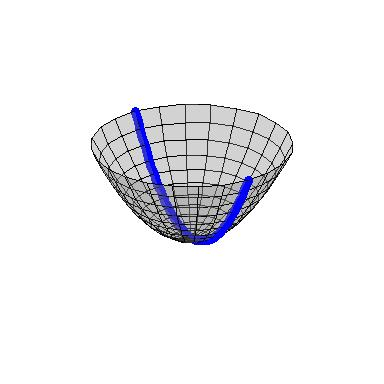
\includegraphics[width=2in]{./ConicsGraphics/Paraboloid01.jpg} & 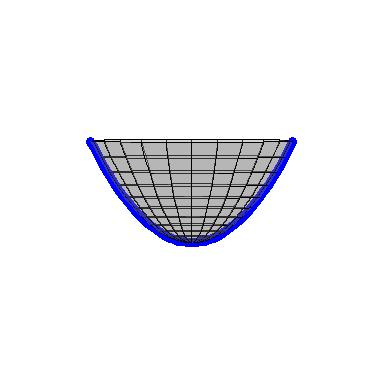
\includegraphics[width=2in]{./ConicsGraphics/Paraboloid02.jpg} \\

\end{tabular}

\end{center}

Every cross section through the vertex of the paraboloid is a parabola with the same focus.  To see why this is important, imagine the dashed lines below as electromagnetic waves heading towards a parabolic dish.   It turns out that the waves reflect off the parabola and concentrate at the focus which then becomes the optimal place for the receiver.  If, on the other hand, we imagine the dashed lines as emanating from the focus, we see that the waves are reflected off the parabola in a coherent fashion as in the case in a flashlight.  Here, the bulb is placed at the focus and the light rays are reflected off a parabolic mirror to give directional light.

\begin{center}

\begin{mfpic}[15]{-5}{7}{-1}{10}
\arrow \reverse \arrow \rotatepath{(0,0), -45}  \function{-6.25,6.25,0.1}{(x**2)/8}
\dashed  \rotatepath{(0,0), -45}   \polyline{(0,2), (2, 0.5), (2, 6)} 
\dashed  \rotatepath{(0,0), -45} \polyline{(0,2), (-2,0.5), (-2, 6)}
\dashed \rotatepath{(0,0), -45}   \polyline{(0,2), (4,2), (4, 6)}
\dashed \rotatepath{(0,0), -45}   \polyline{(0,2), (-4,2), (-4, 6)}
\dashed \rotatepath{(0,0), -45}  \polyline{(0,2), (6,4.5), (6, 6)}
\dashed \rotatepath{(0,0), -45}  \polyline{(0,2), (-6,4.5), (-6, 6)}
\plotsymbol[3pt]{Asterisk}{(1.414, 1.414)}
\tlabel[cc](2, 2){$F$}
\gfill \rotatepath{(0,0), -45}  \circle{(2,0.5),0.07}
\gfill \rotatepath{(0,0), -45}  \circle{(-2,0.5),0.07}
\gfill \rotatepath{(0,0), -45}  \circle{(4,2),0.07}
\gfill \rotatepath{(0,0), -45}  \circle{(-4,2),0.07}
\gfill \rotatepath{(0,0), -45} \circle{(6,4.5),0.07}
\gfill \rotatepath{(0,0), -45} \circle{(-6,4.5),0.07}
\end{mfpic}

\end{center}

\begin{ex} A satellite dish is to be constructed in the shape of a paraboloid of revolution.  If the receiver placed at the focus is located 2 ft above the vertex of the dish, and the dish is to be 12 feet wide, how deep will the dish be?

\medskip

{\bf Solution.}  One way to approach this problem is to determine the equation of the parabola suggested to us by this data.  For simplicity, we'll assume the vertex is $(0,0)$ and the parabola opens upwards.  Our standard form for such a parabola is $x^2 = 4py$.  Since the focus is $2$ units above the vertex, we know  $p=2$, so we have $x^2 = 8y$.  Visually,

\begin{center}

\begin{mfpic}[25]{-7}{7}{0}{5}
\axes
\xmarks{-6, -5, -4, -3, -2, -1, 0,1,2,3,4,5,6}
\ymarks{0,1,2,3,4}
\point[3pt]{(0,0)}
\point[3pt]{(6,36/8)}
\point[3pt]{(-6,36/8)}
\arrow \function{-6.25,6.25,0.1}{(x**2)/8}
\arrow \function{6.25,-6.25,0.1}{(x**2)/8}
\arrow \polyline{(-5.5, 4.5),(5.5,4.5)}
\arrow \polyline{(5.5,4.5), (-5.5, 4.5)}
\arrow \polyline{(6, 0.5),(6,4)}
\arrow \polyline{(6,4), (6,0.5)}
\plotsymbol[3pt]{Asterisk}{(0, 2)}
\tlabel[cc](6.25,2.25){?}
\tlabel(6.25, 4.25){$(6,y)$}
\tlabel(0.25,5){$y$}
\tlabel(7, -0.25){$x$}
\gclear \tlabelrect[cc](0,4){$12$ units wide}
\tlpointsep{4pt}
\small
\axislabels {x}{{$-6 \hspace{7pt}$} -6, {$6$} 6}
\axislabels {y}{{$2$} 2}
\normalsize
\end{mfpic}

\end{center}

Since the parabola is $12$ feet wide, we know the edge is $6$ feet from the vertex.  To find the depth, we are looking for the $y$ value when $x=6$.  Substituting $x=6$ into the equation of the parabola yields $6^2 = 8y$ or $y = \frac{36}{8} = \frac{9}{2} = 4.5$.  Hence, the dish will be  $4.5$ feet deep.  \qed

\end{ex}

\newpage

\subsection{Exercises}


In Exercises \ref{parabolasketchfirst} - \ref{parabolasketchlast}, sketch the graph of the given parabola.  Find the vertex, focus and directrix.  Include the endpoints of the latus rectum in your sketch.

\begin{multicols}{2}
\begin{enumerate}

\item $(x - 3)^{2} = -16y$ \label{parabolasketchfirst}
\item $\left(x + \frac{7}{3}\right)^{2} = 2\left(y + \frac{5}{2}\right)$


\setcounter{HW}{\value{enumi}}
\end{enumerate}
\end{multicols}

\begin{multicols}{2}
\begin{enumerate}
\setcounter{enumi}{\value{HW}}


\item $(y - 2)^{2} = -12(x + 3)$ 
\item $(y + 4)^{2} = 4x$

\setcounter{HW}{\value{enumi}}
\end{enumerate}
\end{multicols}

\begin{multicols}{2}
\begin{enumerate}
\setcounter{enumi}{\value{HW}}


\item $(x-1)^2 = 4(y+3)$
\item $(x+2)^2 = -20(y-5)$


\setcounter{HW}{\value{enumi}}
\end{enumerate}
\end{multicols}

\begin{multicols}{2}
\begin{enumerate}
\setcounter{enumi}{\value{HW}}

\item $(y-4)^2 = 18(x-2)$
\item $\left(y+ \frac{3}{2}\right)^2 = -7 \left(x+ \frac{9}{2}\right)$ \label{parabolasketchlast}


\setcounter{HW}{\value{enumi}}
\end{enumerate}
\end{multicols}



In Exercises \ref{stdfrmparabolafirst} - \ref{stdfrmparabolalast}, put the equation into standard form and identify the vertex, focus and directrix.

\begin{multicols}{2}
\begin{enumerate}
\setcounter{enumi}{\value{HW}}

\item $y^{2} - 10y - 27x + 133 = 0$ \label{stdfrmparabolafirst}
\item $25x^{2} + 20x + 5y - 1 = 0$

\setcounter{HW}{\value{enumi}}
\end{enumerate}
\end{multicols}

\begin{multicols}{2}
\begin{enumerate}
\setcounter{enumi}{\value{HW}}

\item $x^2 + 2x - 8y + 49 = 0$
\item $2y^2 + 4y +x - 8 = 0$

\setcounter{HW}{\value{enumi}}
\end{enumerate}
\end{multicols}

\begin{multicols}{2}
\begin{enumerate}
\setcounter{enumi}{\value{HW}}

\item $x^2-10x+12y+1=0$
\item  $3y^2-27y+4x+\frac{211}{4} = 0$ \label{stdfrmparabolalast}

\setcounter{HW}{\value{enumi}}
\end{enumerate}
\end{multicols}


In Exercises \ref{buildparafirst} - \ref{buildparalast}, find an equation for the parabola which fits the given criteria.

\begin{multicols}{2}
\begin{enumerate}
\setcounter{enumi}{\value{HW}}

\item Vertex $(7, 0)$, focus $(0, 0)$ \label{buildparafirst}
\item Focus $(10, 1)$, directrix $x = 5$


\setcounter{HW}{\value{enumi}}
\end{enumerate}
\end{multicols}

\begin{multicols}{2}
\begin{enumerate}
\setcounter{enumi}{\value{HW}}


\item Vertex $(-8, -9)$; $(0, 0)$ and $(-16, 0)$ are points on the curve
\item The endpoints of latus rectum are $(-2, -7)$ and $(4, -7)$ \label{buildparalast}

\setcounter{HW}{\value{enumi}}
\end{enumerate}
\end{multicols}

\begin{enumerate}
\setcounter{enumi}{\value{HW}}

\item  The mirror in Carl's flashlight is a paraboloid of revolution.  If the mirror is 5 centimeters in diameter and 2.5 centimeters deep, where should the light bulb be placed so it is at the focus of the mirror?

\item  A parabolic Wi-Fi antenna is constructed by taking a flat sheet of metal and bending it into a parabolic shape.\footnote{This shape is called a `parabolic cylinder.'}  If the cross section of the antenna is a parabola which is 45 centimeters wide and 25 centimeters deep, where should the receiver be placed to maximize reception?

\item  \label{parabolaarch} A parabolic arch is constructed which is 6 feet wide at the base and 9 feet tall in the middle. Find the height of the arch exactly 1 foot in from the base of the arch. 

\item  A popular novelty item is the `mirage bowl.'  Follow this  \href{http://spie.org/etop/2007/etop07methodsV.pdf}{\underline{link}} to see another startling application of the reflective property of the parabola.

\item With the help of your classmates, research spinning liquid mirrors.  To get you started, check out this \href{http://www.astro.ubc.ca/LMT/lzt/}{\underline{website}}.

\end{enumerate}

\newpage

\subsection{Answers}

\begin{enumerate}

\item \begin{multicols}{2}
{\small $(x - 3)^{2} = -16y$}\\
{\small Vertex $(3, 0)$}\\
{\small Focus $(3, -4)$}\\
{\small Directrix $y = 4$}\\
{\small Endpoints of latus rectum $(-5, -4)$, $(11, -4)$}\\

\vfill

\columnbreak

\begin{mfpic}[10]{-6}{12}{-5}{5}
\axes
\xmarks{-5 step 1 until 11}
\ymarks{-4 step 1 until 4}
\arrow \reverse \arrow \function{-5.5,11.5,0.1}{((x - 3)**2)/(-16)}
\arrow \reverse \arrow \polyline{(-6,4),(12,4)}
\plotsymbol[3pt]{Asterisk}{(3,-4)}
\tlabel(12,-0.5){\scriptsize $x$}
\tlabel(0.5,5){\scriptsize $y$}
\point[3pt]{(3,0),(-5,-4),(11,-4)}
\tlpointsep{4pt}
\tiny
\axislabels {x}{{$-5 \hspace{7pt}$} -5, {$-4 \hspace{7pt}$} -4, {$-3 \hspace{7pt}$} -3, {$-2 \hspace{7pt}$} -2, {$-1 \hspace{7pt}$} -1, {$1$} 1, {$2$} 2, {$3$} 3, {$4$} 4, {$5$} 5, {$6$} 6, {$7$} 7, {$8$} 8, {$9$} 9, {$10$} 10, {$11$} 11}
\axislabels {y}{{$-4$} -4, {$-3$} -3, {$-2$} -2, {$-1$} -1, {$1$} 1, {$2$} 2, {$3$} 3, {$4$} 4}
\normalsize
\end{mfpic}
\end{multicols}

\smallskip

\item  \begin{multicols}{2}
{\small $\left(x + \frac{7}{3}\right)^{2} = 2\left(y + \frac{5}{2}\right)$}\\
{\small Vertex $\left(-\frac{7}{3}, -\frac{5}{2} \right)$}\\
{\small Focus $\left(-\frac{7}{3}, -2 \right)$}\\
{\small Directrix $y = -3$}\\
{\small Endpoints of latus rectum $\left(-\frac{10}{3}, -2 \right)$, $\left(-\frac{4}{3}, -2 \right)$}\\

\vfill

\columnbreak


\begin{mfpic}[15][20]{-6}{1}{-4}{3}
\axes
\xmarks{-5 step 1 until 0}
\ymarks{-3 step 1 until 2}
\arrow \reverse \arrow \function{-5.5,0.8,0.1}{((x + (7/3))**2)/2 - (5/2)}
\arrow \reverse \arrow \polyline{(-5,-3),(1,-3)}
\plotsymbol[3pt]{Asterisk}{(-2.333,-2)}
\tlabel(1,-0.5){\scriptsize $x$}
\tlabel(0.5,3){\scriptsize $y$}
\point[3pt]{(-2.333,-2.5),(-3.333,-2),(-1.333,-2)}
\tlpointsep{4pt}
\tiny
\axislabels {x}{{$-5 \hspace{7pt}$} -5, {$-4 \hspace{7pt}$} -4, {$-3 \hspace{7pt}$} -3, {$-2 \hspace{7pt}$} -2, {$-1 \hspace{7pt}$} -1}
\axislabels {y}{{$-3$} -3, {$-2$} -2, {$-1$} -1, {$1$} 1, {$2$} 2}
\normalsize
\end{mfpic}
\end{multicols}

\smallskip

\item \begin{multicols}{2} 

{\small $(y - 2)^{2} = -12(x + 3)$} \\
{\small Vertex $(-3, 2)$} \\
{\small Focus $(-6, 2)$} \\
{\small Directrix $x = 0$}\\
{\small Endpoints of latus rectum $(-6, 8)$, $(-6, -4)$}\\

\vfill

\columnbreak


\begin{mfpic}[10]{-8}{1}{-5}{9}
\axes
\xmarks{-7 step 1 until 0}
\ymarks{-4 step 1 until 8}
\arrow \reverse \function{-6.8,-3,0.1}{2+sqrt((-12*x) - 36)}
\arrow \reverse \function{-6.8,-3,0.1}{2-sqrt((-12*x) - 36)}
\plotsymbol[3pt]{Asterisk}{(-6,2)}
\tlabel(1,-0.5){\scriptsize $x$}
\tlabel(0.5,9){\scriptsize $y$}
\point[3pt]{(-3,2),(-6,-4),(-6,8)}
\tlpointsep{4pt}
\tiny
\axislabels {x}{{$-7 \hspace{7pt}$} -7, {$-6 \hspace{7pt}$} -6, {$-5 \hspace{7pt}$} -5, {$-4 \hspace{7pt}$} -4, {$-3 \hspace{7pt}$} -3, {$-2 \hspace{7pt}$} -2, {$-1 \hspace{7pt}$} -1}
\axislabels {y}{{$-4$} -4, {$-3$} -3, {$-2$} -2, {$-1$} -1, {$1$} 1, {$2$} 2, {$3$} 3, {$4$} 4, {$5$} 5, {$6$} 6, {$7$} 7, {$8$} 8}
\normalsize
\end{mfpic}
\end{multicols}

\pagebreak

\item \begin{multicols}{2} 
{\small $(y + 4)^{2} = 4x$}\\
{\small Vertex $(0,-4)$} \\
{\small Focus $(1,-4)$} \\
{\small Directrix $x = -1$}\\
{\small Endpoints of latus rectum $(1, -2)$, $(1, -6)$}\\

\vfill

\columnbreak


\begin{mfpic}[15]{-2}{5}{-9}{1}
\axes
\xmarks{-1 step 1 until 4}
\ymarks{-8 step 1 until 0}
\arrow \function{0,5,0.1}{-4-(2*sqrt(x))}
\arrow \function{0,5,0.1}{-4+(2*sqrt(x))}
\arrow \reverse \arrow \polyline{(-1,-9),(-1,1)}
\plotsymbol[3pt]{Asterisk}{(1,-4)}
\tlabel(5,-0.5){\scriptsize $x$}
\tlabel(0.5,1){\scriptsize $y$}
\point[3pt]{(0,-4),(1,-2),(1,-6)}
\tlpointsep{4pt}
\tiny
\axislabels {x}{{$-1 \hspace{7pt}$} -1, {$1$} 1, {$2$} 2, {$3$} 3, {$4$} 4}
\axislabels {y}{{$-8$} -8, {$-7$} -7, {$-6$} -6, {$-5$} -5, {$-4$} -4, {$-3$} -3, {$-2$} -2, {$-1$} -1}
\normalsize
\end{mfpic}
\end{multicols}

\smallskip


\item  \begin{multicols}{2}
{\small $(x-1)^2 = 4(y+3)$}\\
{\small Vertex $\left(1, -3\right)$}\\
{\small Focus $\left(1, -2 \right)$}\\
{\small Directrix $y = -4$}\\
{\small Endpoints of latus rectum $\left(3, -2 \right)$, $\left(-1, -2 \right)$}\\

\vfill

\columnbreak


\begin{mfpic}[15]{-4}{5}{-5}{1}
\axes
\xmarks{-3 step 1 until 4}
\ymarks{-4 step 1 until 0}
\arrow \reverse \arrow \function{-3,5,0.1}{((x -1)**2)/4 - 3}
\arrow \reverse \arrow \polyline{(-5,-4),(5,-4)}
\plotsymbol[3pt]{Asterisk}{(1,-2)}
\tlabel(5,-0.5){\scriptsize $x$}
\tlabel(0.5,1){\scriptsize $y$}
\point[3pt]{(3,-2),(1,-3),(-1,-2)}
\tlpointsep{4pt}
\tiny
\axislabels {x}{{$-3 \hspace{7pt}$} -3, {$-2 \hspace{7pt}$} -2, {$-1 \hspace{7pt}$} -1, {$1$} 1, {$2$} 2, {$3$} 3, {$4$} 4}
\axislabels {y}{{$-4$} -4, {$-3$} -3, {$-2$} -2, {$-1$} -1}
\normalsize
\end{mfpic}
\end{multicols}

\smallskip

\item \begin{multicols}{2}
{\small $(x+2)^2 = -20(y-5)$}\\
{\small Vertex $\left(-2, 5\right)$}\\
{\small Focus $\left(-2, 0 \right)$}\\
{\small Directrix $y = 10$}\\
{\small Endpoints of latus rectum $\left(-12, 0 \right)$, $\left(8, 0 \right)$}\\

\vfill

\columnbreak


\begin{mfpic}[7.5][10]{-13}{9}{-1}{11}
\axes
\xmarks{-12 step 1 until 8}
\ymarks{1 step 1 until 10}
\arrow \reverse \arrow \function{-13,9,0.1}{((x +2)**2)/(0-20) + 5}
\arrow \reverse \arrow \polyline{(-13,10),(9,10)}
\plotsymbol[3pt]{Asterisk}{(-2,0)}
\tlabel(9,-0.5){\scriptsize $x$}
\tlabel(0.5,11){\scriptsize $y$}
\point[3pt]{(-12,0),(-2,5),(8,0)}
\tlpointsep{4pt}
\tiny
\axislabels {x}{{$-12 \hspace{7pt}$} -12,  {$-10 \hspace{7pt}$} -10, {$-8 \hspace{7pt}$} -8, {$-6 \hspace{7pt}$} -6, {$-4 \hspace{7pt}$} -4,  {$-2 \hspace{7pt}$} -2, {$2$} 2,  {$4$} 4,  {$6$} 6, {$8$} 8}
\axislabels {y}{{$1$} 1, {$2$} 2, {$3$} 3, {$4$} 4, {$5$} 5, {$6$} 6, {$7$} 7, {$8$} 8, {$9$} 9, {$10$} 10}
\normalsize
\end{mfpic}
\end{multicols}

\smallskip


\item \begin{multicols}{2}
{\small $(y-4)^2 = 18(x-2)$}\\
{\small Vertex $\left(2, 4\right)$}\\
{\small Focus $\left( \frac{13}{2}, 4 \right)$}\\
{\small Directrix $x = -\frac{5}{2}$}\\
{\small Endpoints of latus rectum $\left(\frac{13}{2}, -5 \right)$, $\left(\frac{13}{2}, 13 \right)$}\\

\vfill

\columnbreak


\begin{mfpic}[15][7.5]{-3}{8}{-6}{14}
\axes
\xmarks{-2 step 1 until 7}
\ymarks{-5 step 1 until 13}
\arrow \function{2,8,0.1}{4+(sqrt(18*(x-2)))}
\arrow \function{2,8,0.1}{4-(sqrt(18*(x-2)))}
\arrow \reverse \arrow \polyline{(-2.5,-6),(-2.5,14)}
\plotsymbol[3pt]{Asterisk}{(6.5,4)}
\tlabel(8,-0.5){\scriptsize $x$}
\tlabel(0.5,14){\scriptsize $y$}
\point[3pt]{(6.5,-5),(2,4),(6.5,13)}
\tlpointsep{4pt}
\tiny
\axislabels {x}{{$-1$} -1, {$1$} 1,  {$2$} 2,  {$3$} 3, {$4$} 4, {$5$} 5,  {$6$} 6,  {$7$} 7}
\axislabels {y}{{$-5$} -5, {$-3$} -3, {$-1$} -1, {$1$} 1, {$3$} 3, {$5$} 5, {$7$} 7, {$9$} 9, {$11$} 11, {$13$} 13}
\normalsize
\end{mfpic}
\end{multicols}

\smallskip

\item \begin{multicols}{2} 
{\small $\left(y+ \frac{3}{2}\right)^2 = -7 \left(x+ \frac{9}{2}\right)$}\\
{\small Vertex $\left(-\frac{9}{2}, -\frac{3}{2}\right)$}\\
{\small Focus $\left( -\frac{25}{4}, -\frac{3}{2} \right)$}\\
{\small Directrix $x = -\frac{11}{4}$}\\
{\small Endpoints of latus rectum $\left(-\frac{25}{4}, 2 \right)$, $\left(-\frac{25}{4}, -5 \right)$}\\

\vfill

\columnbreak


\begin{mfpic}[15]{-7}{1}{-6}{3}
\axes
\xmarks{-6 step 1 until -1}
\ymarks{-5 step 1 until 2}
\arrow \function{-4.5,-7,0.1}{0-1.5+(sqrt((0-7)*(x+4.5)))}
\arrow \function{-4.5,-7,0.1}{0-1.5-(sqrt((0-7)*(x+4.5)))}
\arrow \reverse \arrow \polyline{(-2.75,-6),(-2.75,3)}
\plotsymbol[3pt]{Asterisk}{(-6.25,-1.5)}
\tlabel(1,-0.5){\scriptsize $x$}
\tlabel(0.5,3){\scriptsize $y$}
\point[3pt]{(-6.25,-5),(-4.5,-1.5),(-6.25,2)}
\tlpointsep{4pt}
\tiny
\axislabels {x}{{$-5 \hspace{7pt}$} -5,{$-4 \hspace{7pt}$} -4,{$-3 \hspace{7pt}$} -3,{$-2 \hspace{7pt}$} -2,{$-1 \hspace{7pt}$} -1}
\axislabels {y}{{$-5$} -5, {$-4$} -4, {$-3$} -3, {$-2$} -2, {$-1$} -1, {$1$} 1, {$2$} 2}
\normalsize
\end{mfpic}
\end{multicols}

\setcounter{HW}{\value{enumi}}
\end{enumerate}

\begin{multicols}{2}
\begin{enumerate}
\setcounter{enumi}{\value{HW}}


\item $(y - 5)^{2} = 27(x - 4)$\\
Vertex $(4, 5)$\\
Focus $\left( \frac{43}{4}, 5 \right)$\\
Directrix $x = -\frac{11}{4}$

\item $\left(x + \frac{2}{5} \right)^{2} = -\frac{1}{5}(y - 1)$\\
Vertex $\left( -\frac{2}{5}, 1 \right)$\\
Focus $\left( -\frac{2}{5}, \frac{19}{20} \right)$\\
Directrix $y = \frac{21}{20}$

\setcounter{HW}{\value{enumi}}
\end{enumerate}
\end{multicols}

\begin{multicols}{2}
\begin{enumerate}
\setcounter{enumi}{\value{HW}}


\item  $(x+1)^2=8(y-6)$ \\
Vertex $(-1,6)$\\
Focus $(-1,8)$ \\
Directrix $y=4$

\item  $(y+1)^2=-\frac{1}{2}(x-10)$\\
Vertex $(10,-1)$\\
Focus $\left(\frac{79}{8}, -1 \right)$\\
Directrix $x = \frac{81}{8}$

\setcounter{HW}{\value{enumi}}
\end{enumerate}
\end{multicols}

\begin{multicols}{2}
\begin{enumerate}
\setcounter{enumi}{\value{HW}}

\item $(x-5)^2 = -12(y-2)$\\
Vertex $(5,2)$\\
Focus $(5,-1)$ \\
Directrix $y=5$


\item  $\left(y-\frac{9}{2}\right)^2 = -\frac{4}{3} (x-2)$\\
Vertex $\left(2, \frac{9}{2}\right)$\\
Focus $\left(\frac{5}{3}, \frac{9}{2}\right)$\\
Directrix $x = \frac{7}{3}$

\setcounter{HW}{\value{enumi}}
\end{enumerate}
\end{multicols}

\begin{multicols}{2}
\begin{enumerate}
\setcounter{enumi}{\value{HW}}

\item $y^{2} = -28(x - 7)$
\item $(y - 1)^{2} = 10\left(x - \frac{15}{2} \right)$


\setcounter{HW}{\value{enumi}}
\end{enumerate}
\end{multicols}

\begin{multicols}{2}
\begin{enumerate}
\setcounter{enumi}{\value{HW}}

\item $(x + 8)^{2} = \frac{64}{9}(y + 9)$
\item $(x - 1)^{2} = 6\left(y + \frac{17}{2}\right)$ or\\
$(x - 1)^{2} = -6\left(y + \frac{11}{2}\right)$

\setcounter{HW}{\value{enumi}}
\end{enumerate}
\end{multicols}

\begin{enumerate}
\setcounter{enumi}{\value{HW}}

\item  The bulb should be placed $0.625$ centimeters above the vertex of the mirror. (As verified by Carl himself!)

\item  The receiver should be placed $5.0625$ centimeters from the vertex of the cross section of the antenna.

\item  The arch can be modeled by $x^2=-(y-9)$ or $y=9-x^2$.  One foot in from the base of the arch corresponds to either $x = \pm 2$, so the height is $y=9-(\pm 2)^2=5$ feet.

\end{enumerate}

\closegraphsfile